\section{CHƯƠNG 1: AI VÀ TIỀN XỬ LÝ DỮ LIỆU - NỀN TẢNG CỦA TRÍ TUỆ}

\subsection{Tổng quan về Trí tuệ nhân tạo (AI)}
Trí tuệ nhân tạo (Artificial Intelligence - AI) là lĩnh vực khoa học máy tính tập trung vào việc tạo ra các hệ thống có khả năng thực hiện các nhiệm vụ đòi hỏi trí thông minh của con người. Trong chương này, chúng ta khám phá vai trò sống còn của dữ liệu đối với AI thông qua nguyên lý "Garbage In, Garbage Out".

\subsection{Vai trò của Tiền xử lý dữ liệu trong ML/DL}
Tiền xử lý dữ liệu (Data Preprocessing) là bước chiếm tới 80% thời gian trong một dự án khoa học dữ liệu. Nó bao gồm làm sạch, biến đổi và chuẩn hóa dữ liệu để các thuật toán học máy có thể tối ưu hóa các trọng số một cách hiệu quả nhất.

\subsection{Lý thuyết các kỹ thuật Tiền xử lý Nâng cao}
Bên cạnh các kỹ thuật cơ bản (Mean/Median Imputation, Scaling), chương này đi sâu vào các kỹ thuật đối phó với thách thức thực tế:
\begin{itemize}
    \item \textbf{Robust Scaling:} Sử dụng Median và IQR để chuẩn hóa dữ liệu có nhiều ngoại lai.
    \item \textbf{SMOTE (Synthetic Minority Over-sampling Technique):} Tạo dữ liệu giả lập cho lớp thiểu số để xử lý mất cân bằng.
    \item \textbf{Target Encoding:} Mã hóa các biến phân loại có số lượng nhãn lớn (high cardinality).
    \item \textbf{Feature Derivation:} Tạo các đặc trưng mới từ tri thức lĩnh vực (domain knowledge).
\end{itemize}

\subsection{Thực nghiệm chuyên sâu trên 4 Datasets}

\subsubsection{Dataset 1: Used Car Price (Numerical - Outliers & Feature Derivation)}
\textbf{Thách thức:} Dữ liệu giá xe cũ thường chứa các giá trị ngoại lai cực lớn và các cột dữ liệu thô (năm sản xuất, số dặm).
\textbf{Giải pháp:} Áp dụng RobustScaler và tính toán các đặc trưng mới như "Car Age", "Mileage per Year".
\paragraph{Phân tích bộ dữ liệu Used Car Price} \hfill \\
Bài toán dự báo giá xe cũ (Regression) dựa trên các thuộc tính như năm sản xuất, quãng đường đã đi, nhiên liệu, v.v.

\paragraph{Kỹ thuật xử lý: Feature Derivation và Robust Scaling} \hfill \\
Chúng ta tạo ra biến mới "Car Age" để phản ánh trực tiếp độ cũ của xe thay vì chỉ dùng năm sản xuất. Đồng thời, áp dụng RobustScaler để chuẩn hóa dữ liệu vì giá xe và quãng đường đi được thường có phân phối lệch (skewed) và chứa nhiều giá trị ngoại lai.

\paragraph{Kết quả thực nghiệm} \hfill \\
\begin{figure}[H]
    \centering
    \includegraphics[width=0.7\linewidth]{Chương_1/results/used_car/price_boxplot_before.png}
    \caption{Phân phối giá bán với nhiều giá trị ngoại lai (Outliers)}
    \label{fig:car_outliers}
\end{figure}

Việc sử dụng RobustScaler giúp mô hình hồi quy tuyến tính hoạt động ổn định hơn, không bị chệch hướng bởi các dòng xe hạng sang có giá cực cao.

\begin{figure}[H]
    \centering
    \includegraphics[width=0.7\linewidth]{Chương_1/results/used_car/actual_vs_pred.png}
    \caption{So sánh giữa giá thực tế và giá dự báo}
    \label{fig:car_regression}
\end{figure}


\subsubsection{Dataset 2: Telco Churn (Tabular - Class Imbalance & SMOTE)}
\textbf{Thách thức:} Tỷ lệ khách hàng rời bỏ (Churn) thường thấp hơn nhiều so với khách hàng ở lại, gây ra sai lệch cho mô hình.
\textbf{Giải pháp:} Sử dụng SMOTE để cân bằng dữ liệu và mã hóa One-hot cho các dịch vụ viễn thông.
\paragraph{Phân tích bộ dữ liệu Telco Churn} \hfill \\
Dự báo khả năng khách hàng rời bỏ dịch vụ viễn thông. Đây là bài toán phân loại nhị phân tiêu biểu.

\paragraph{Phân tích biến mục tiêu và các yếu tố ảnh hưởng} \hfill \\
Tỷ lệ khách hàng rời bỏ (Churn) chiếm khoảng 26.5\% dữ liệu, tạo ra sự mất cân bằng nhẹ:
\begin{figure}[H]
    \centering
    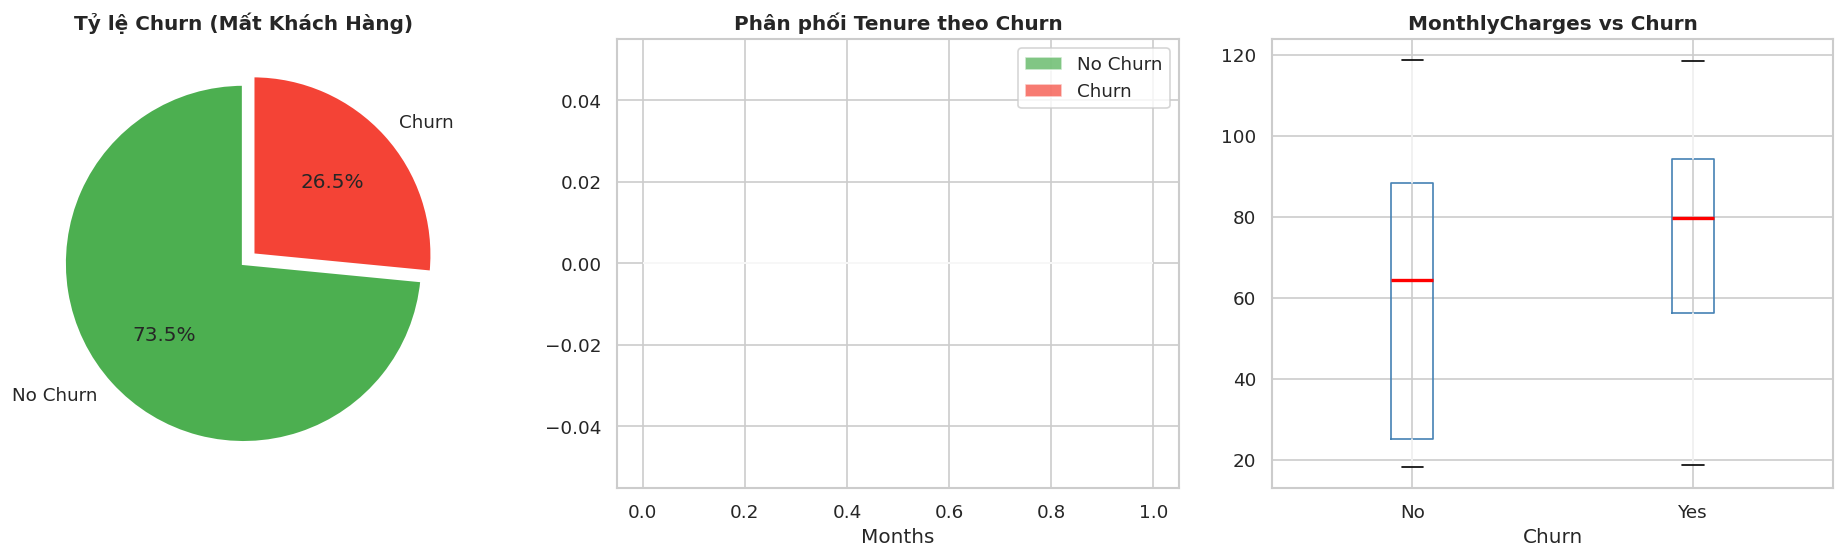
\includegraphics[width=0.8\linewidth]{Chương_1/results/telco/01_churn_eda.png}
    \caption{Phân phối nhãn Churn và thời gian gắn bó (Tenure)}
\end{figure}

Hình 1.9 cho thấy khách hàng mới (Tenure thấp) có xu hướng rời bỏ dịch vụ cao hơn hẳn khách hàng lâu năm. Điều này gợi ý rằng các chương trình khuyến mãi nên tập trung vào giai đoạn đầu của hợp đồng.

Chúng ta quan sát thấy khách hàng sử dụng hợp đồng ngắn hạn (Month-to-month) và thanh toán bằng séc điện tử (Electronic check) có tỷ lệ rời bỏ cao nhất:
\begin{figure}[H]
    \centering
    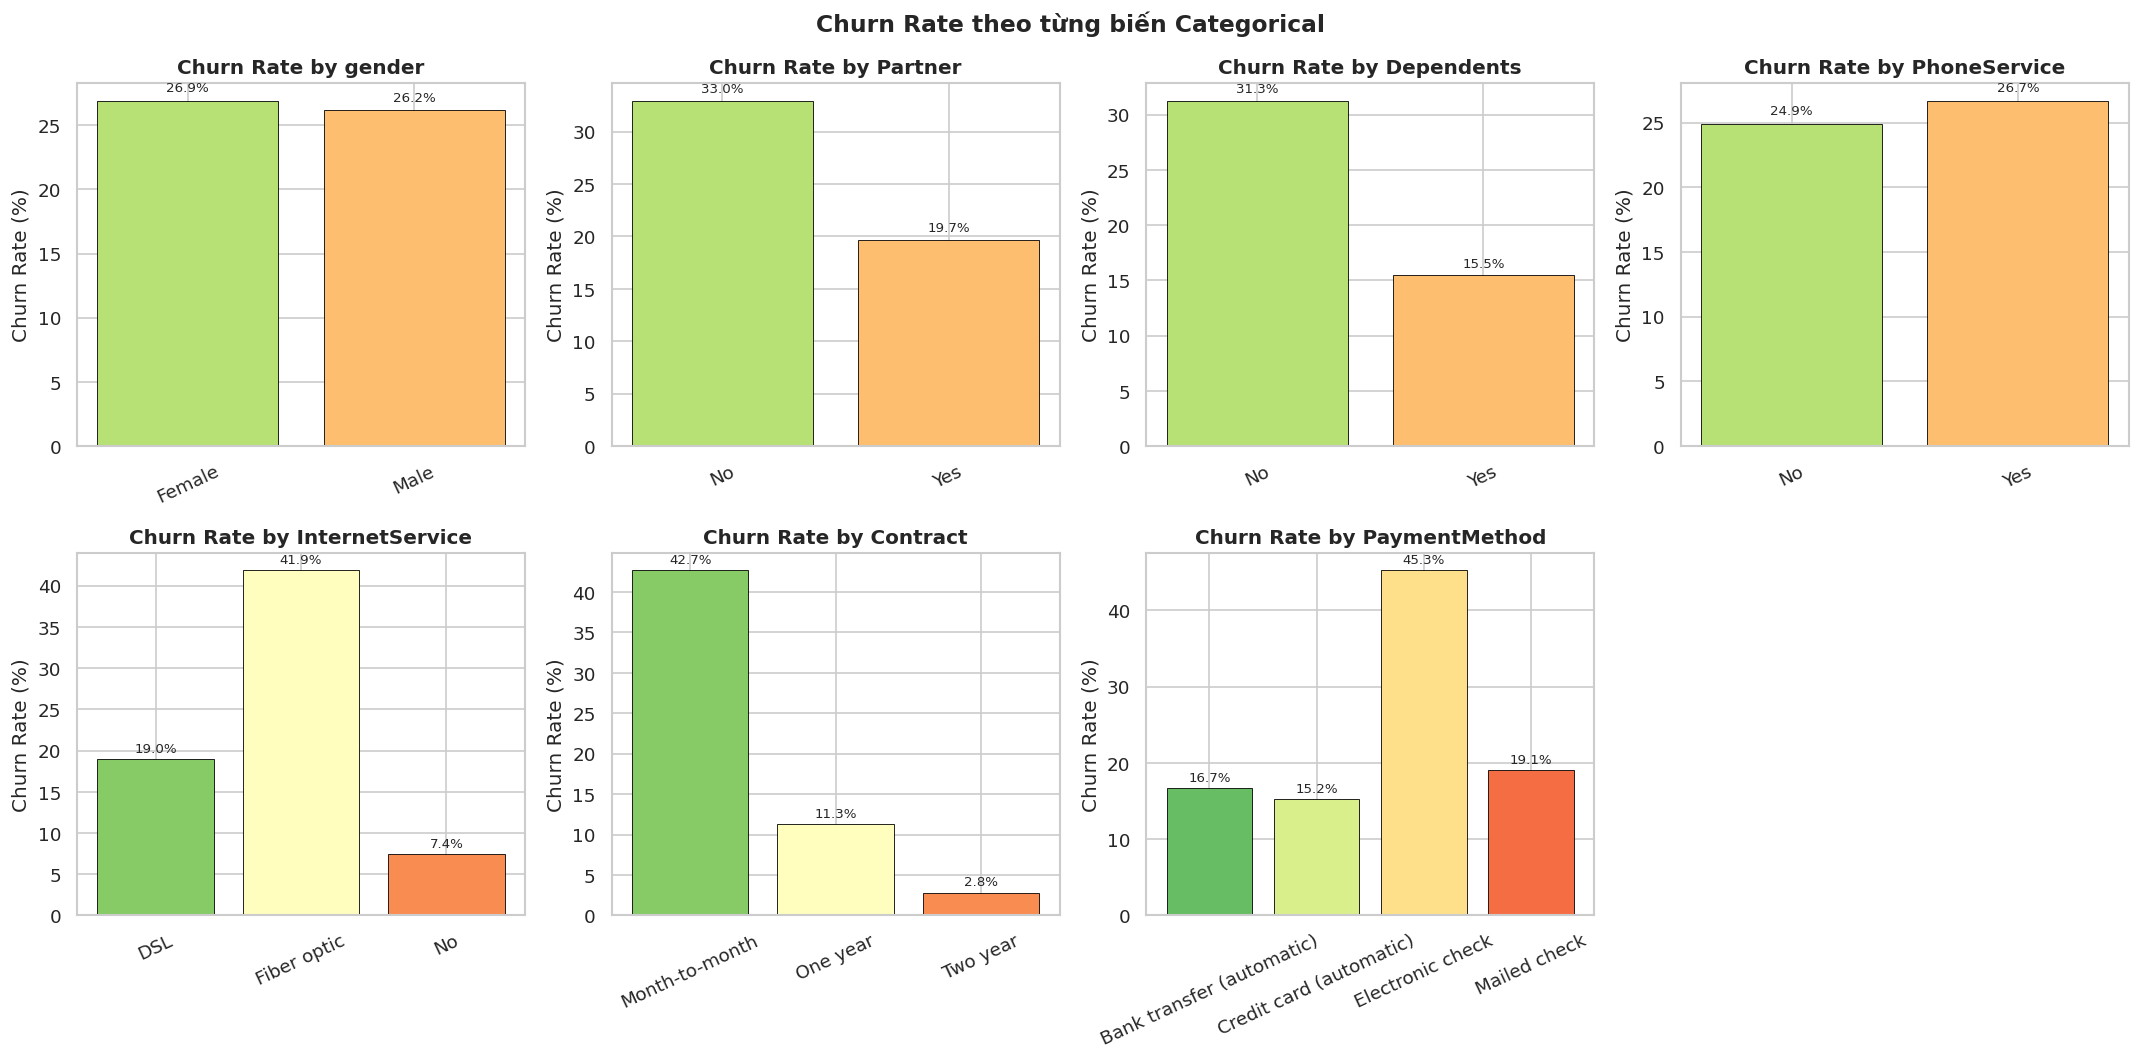
\includegraphics[width=0.8\linewidth]{Chương_1/results/telco/02_churn_by_category.png}
    \caption{Tỷ lệ rời bỏ theo loại hợp đồng và phương thức thanh toán}
\end{figure}

Hình 1.10 chỉ ra rằng loại hợp đồng là yếu tố then chốt: khách hàng "Month-to-month" có rủi ro rời bỏ cao nhất, trong khi hợp đồng 1-2 năm giúp duy trì sự ổn định. Thanh toán qua "Electronic check" cũng là một dấu hiệu cảnh báo cần chú ý.

\paragraph{Kỹ thuật xử lý: Cân bằng dữ liệu với SMOTE} \hfill \\
Để mô hình không bị thiên kiến về lớp đa số, kỹ thuật SMOTE được áp dụng để sinh thêm các mẫu giả lập cho lớp Churn:
\begin{figure}[H]
    \centering
    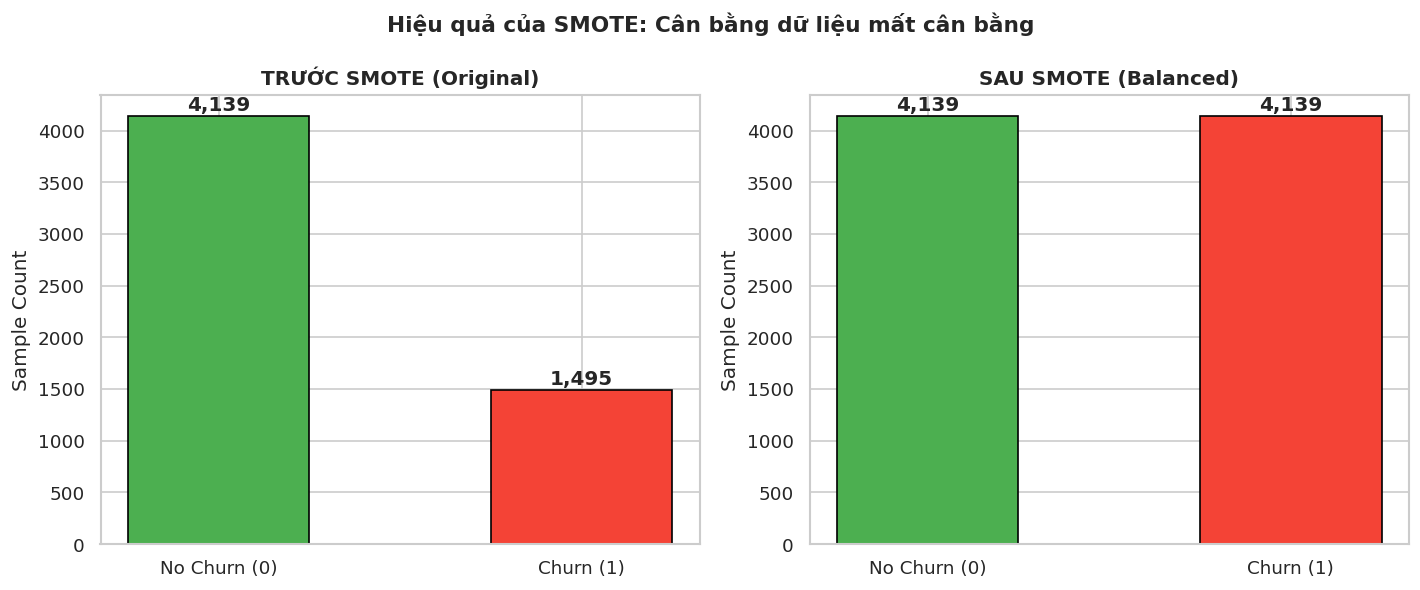
\includegraphics[width=0.8\linewidth]{Chương_1/results/telco/03_smote_comparison.png}
    \caption{Tương quan dữ liệu trước và sau khi áp dụng SMOTE}
\end{figure}

Hình 1.11 minh họa hiệu quả của kỹ thuật SMOTE. Bằng cách sinh thêm các mẫu giả lập cho lớp thiểu số dựa trên khoảng cách K-Nearest Neighbors, chúng ta đã cân bằng được tập huấn luyện, giúp mô hình học được đặc trưng của nhóm khách hàng rời bỏ một cách công bằng hơn.

\paragraph{Kết quả thực nghiệm} \hfill \\
Thực nghiệm sử dụng Logistic Regression và Random Forest với bộ tham số cân bằng.

\begin{table}[H]
    \centering
    \begin{tabular}{|l|c|c|c|c|}
    \hline
    \textbf{Mô hình} & \textbf{Accuracy} & \textbf{ROC-AUC} & \textbf{F1 (Churn)} & \textbf{Recall (Churn)} \\ \hline
    Logistic Regression & 0.7949 & 0.8407 & 0.61 & 0.61 \\ \hline
    Random Forest & 0.7786 & 0.8197 & 0.57 & 0.55 \\ \hline
    \end{tabular}
    \caption{Kết quả phân loại khách hàng rời bỏ}
\end{table}

\begin{figure}[H]
    \centering
    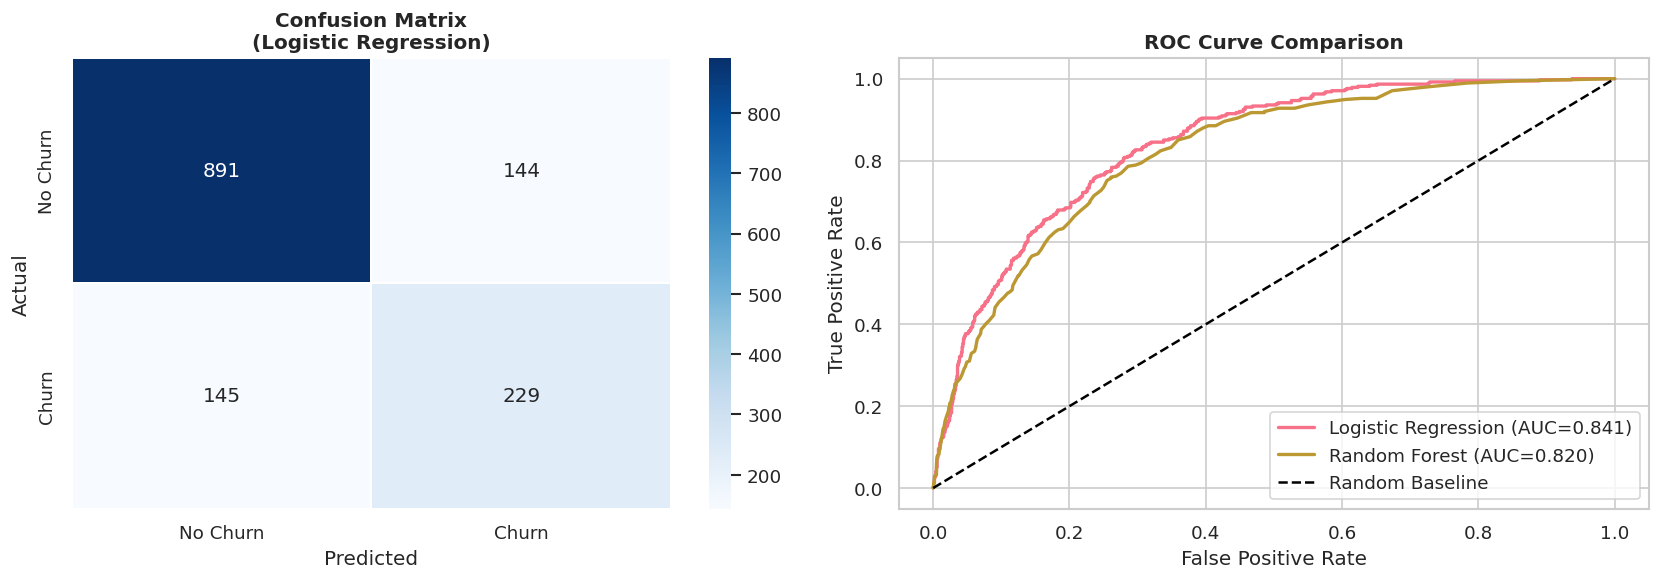
\includegraphics[width=0.8\linewidth]{Chương_1/results/telco/04_confusion_roc.png}
    \caption{Ma trận nhầm lẫn và Đường cong ROC (Logistic Regression chiếm ưu thế)}
\end{figure}

Hình 1.12 cho thấy mô hình Logistic Regression đạt diện tích dưới đường cong (AUC) là 0.84, một con số khá tốt cho bài toán dự báo hành vi con người. Ma trận nhầm lẫn xác nhận khả năng cân bằng giữa việc phát hiện Churn và duy trì độ chính xác tổng thể.

\paragraph{Feature Importance} \hfill \\
Biểu đồ dưới đây chỉ ra các yếu tố "giữ chân" khách hàng hiệu quả nhất:
\begin{figure}[H]
    \centering
    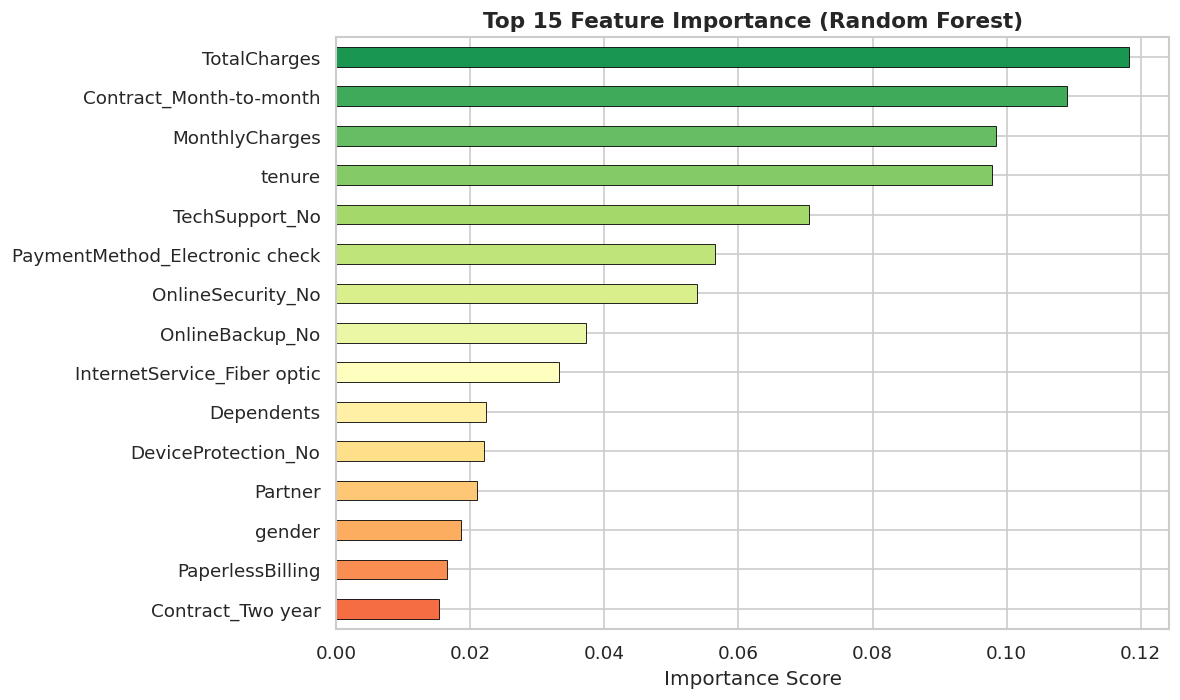
\includegraphics[width=0.8\linewidth]{Chương_1/results/telco/05_feature_importance.png}
    \caption{Tầm quan trọng của các đặc trưng trong bài toán Churn}
\end{figure}

Hình 1.13 tổng kết các đặc trưng quan trọng nhất. Ngoài loại hợp đồng và thời gian gắn bó, tổng số tiền thanh toán (\texttt{TotalCharges}) và loại hình Internet cũng đóng vai trò quyết định trong việc dự báo khả năng khách hàng rời đi.

\paragraph{Phụ lục: Chi tiết quá trình thực hiện thực nghiệm Telco Churn} \hfill \\
Dưới đây là các bước thực hiện chi tiết cho bài toán dự báo khách hàng rời bỏ dịch vụ.

\begin{figure}[H]
    \centering
    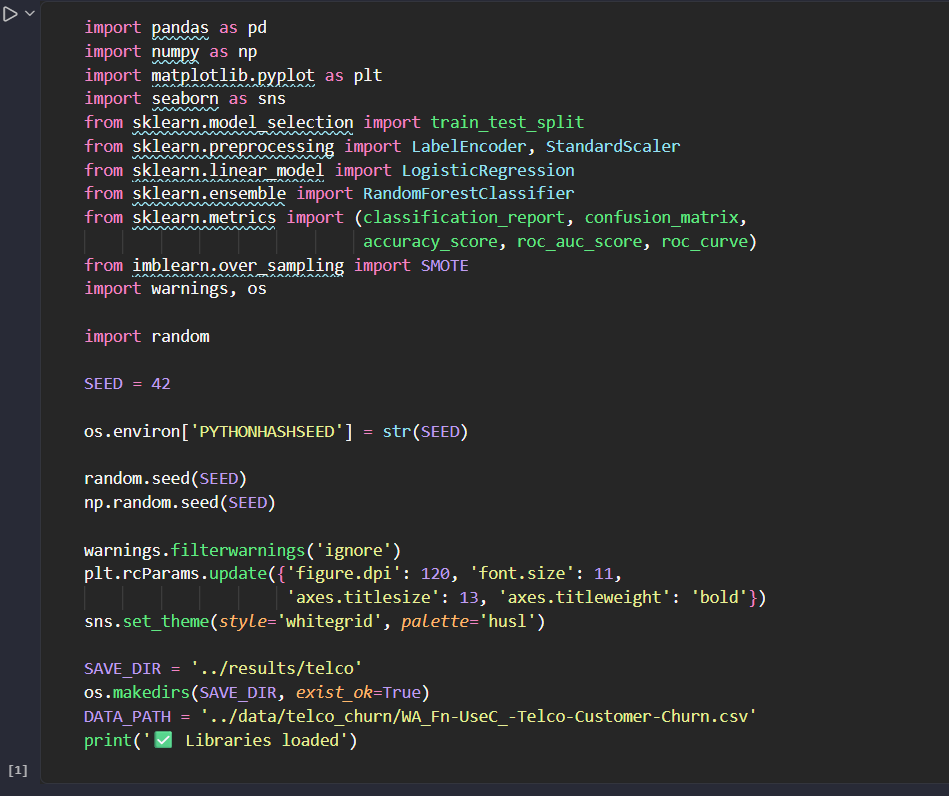
\includegraphics[width=0.9\linewidth]{Chương_1/docs/ch1/28.png}
    \caption{Khởi tạo: Import các thư viện xử lý dữ liệu và học máy cho bài toán phân loại.}
\end{figure}

\begin{figure}[H]
    \centering
    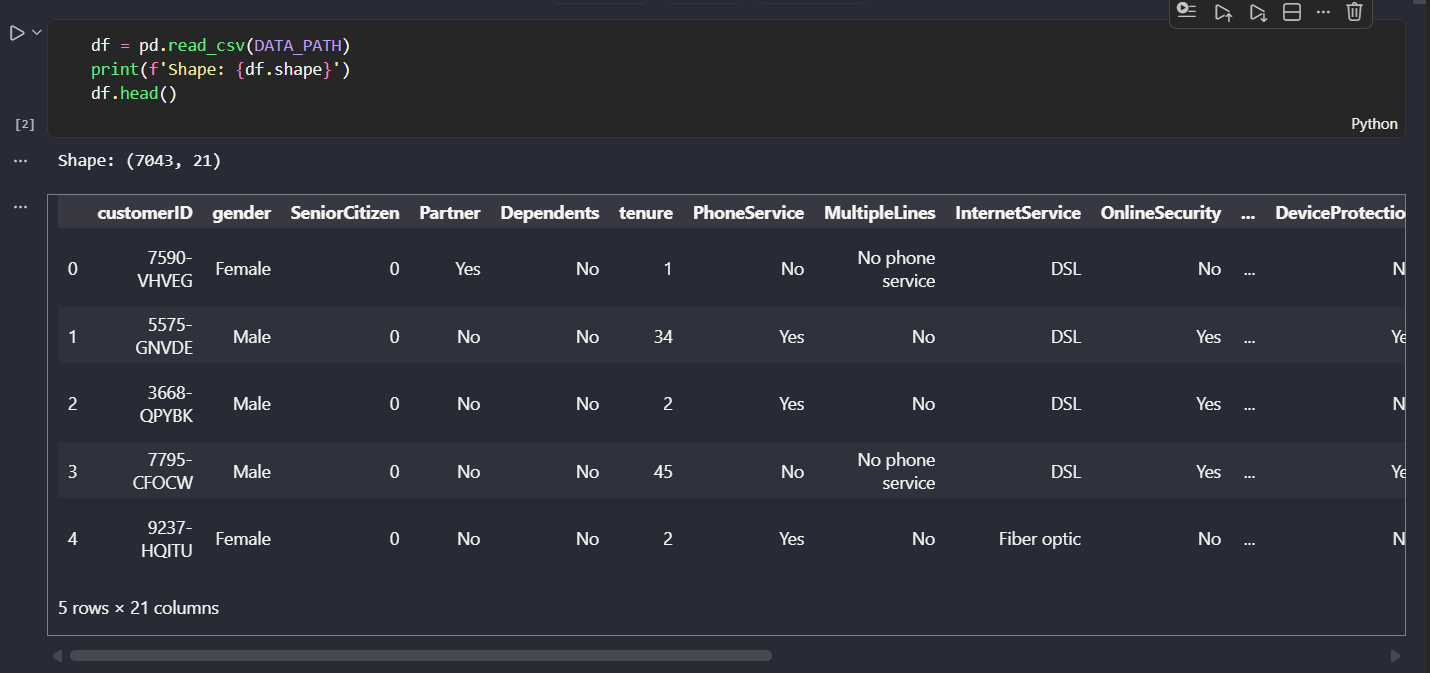
\includegraphics[width=0.9\linewidth]{Chương_1/docs/ch1/29.png}
    \caption{Tải dữ liệu Telco Churn: Đọc dữ liệu và kiểm tra phân phối của biến mục tiêu Churn.}
\end{figure}

\begin{figure}[H]
    \centering
    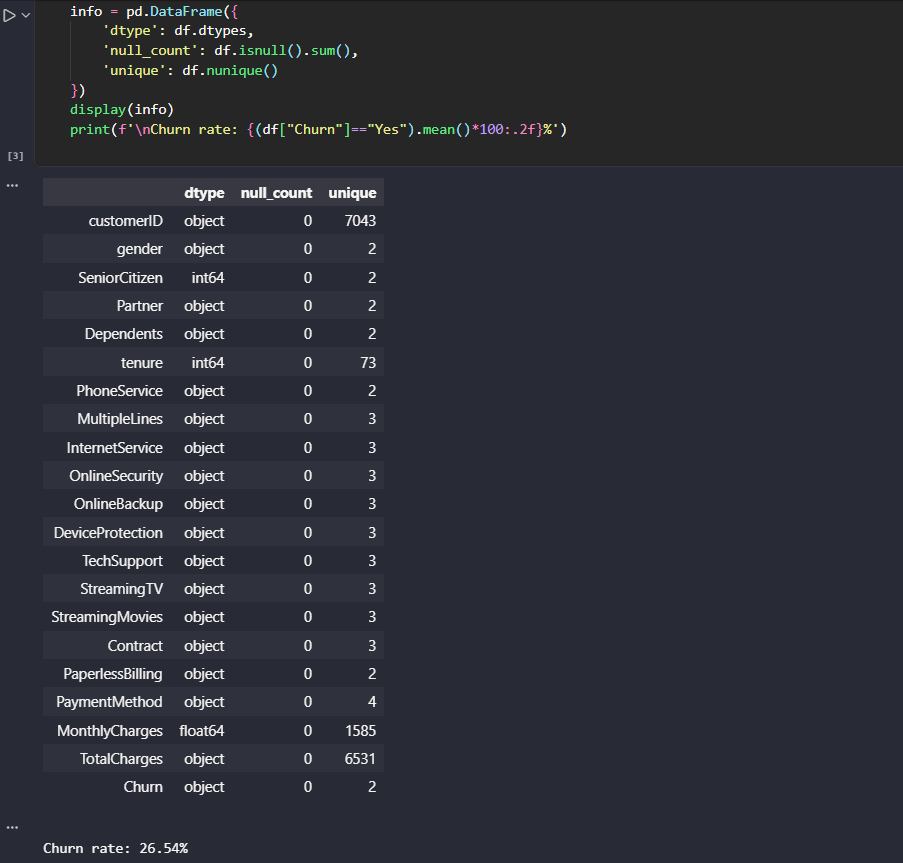
\includegraphics[width=0.9\linewidth]{Chương_1/docs/ch1/30.png}
    \caption{Thống kê cơ bản: Xem xét kiểu dữ liệu và tỷ lệ khách hàng rời bỏ (26.54\%).}
\end{figure}

\begin{figure}[H]
    \centering
    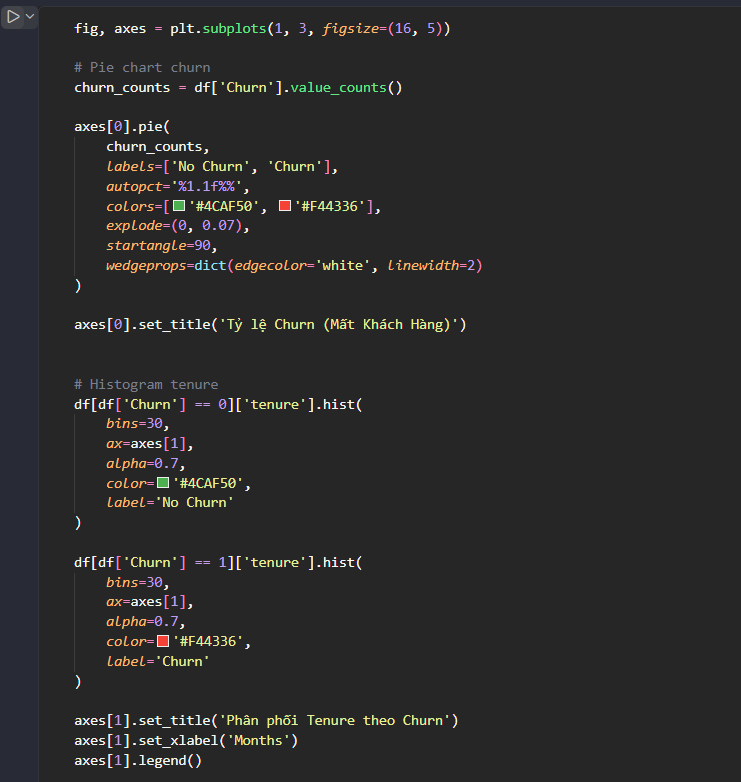
\includegraphics[width=0.9\linewidth]{Chương_1/docs/ch1/31.png}
    \caption{Mã nguồn EDA (Phần 1): Vẽ biểu đồ tròn tỷ lệ Churn và biểu đồ histogram cho Tenure.}
\end{figure}

\begin{figure}[H]
    \centering
    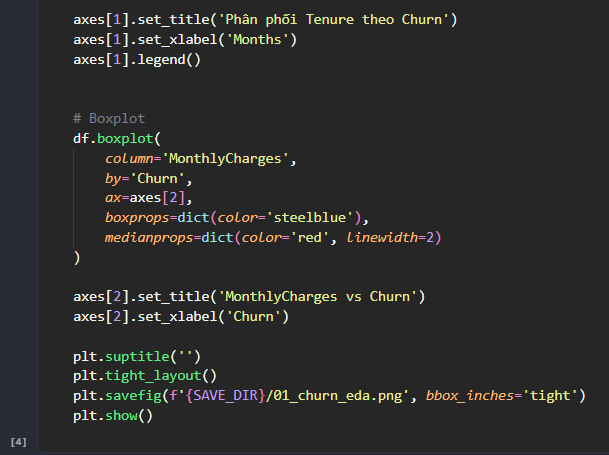
\includegraphics[width=0.9\linewidth]{Chương_1/docs/ch1/32.png}
    \caption{Mã nguồn EDA (Phần 2): Bổ sung biểu đồ Boxplot cho chi phí hàng tháng (Monthly Charges).}
\end{figure}

\begin{figure}[H]
    \centering
    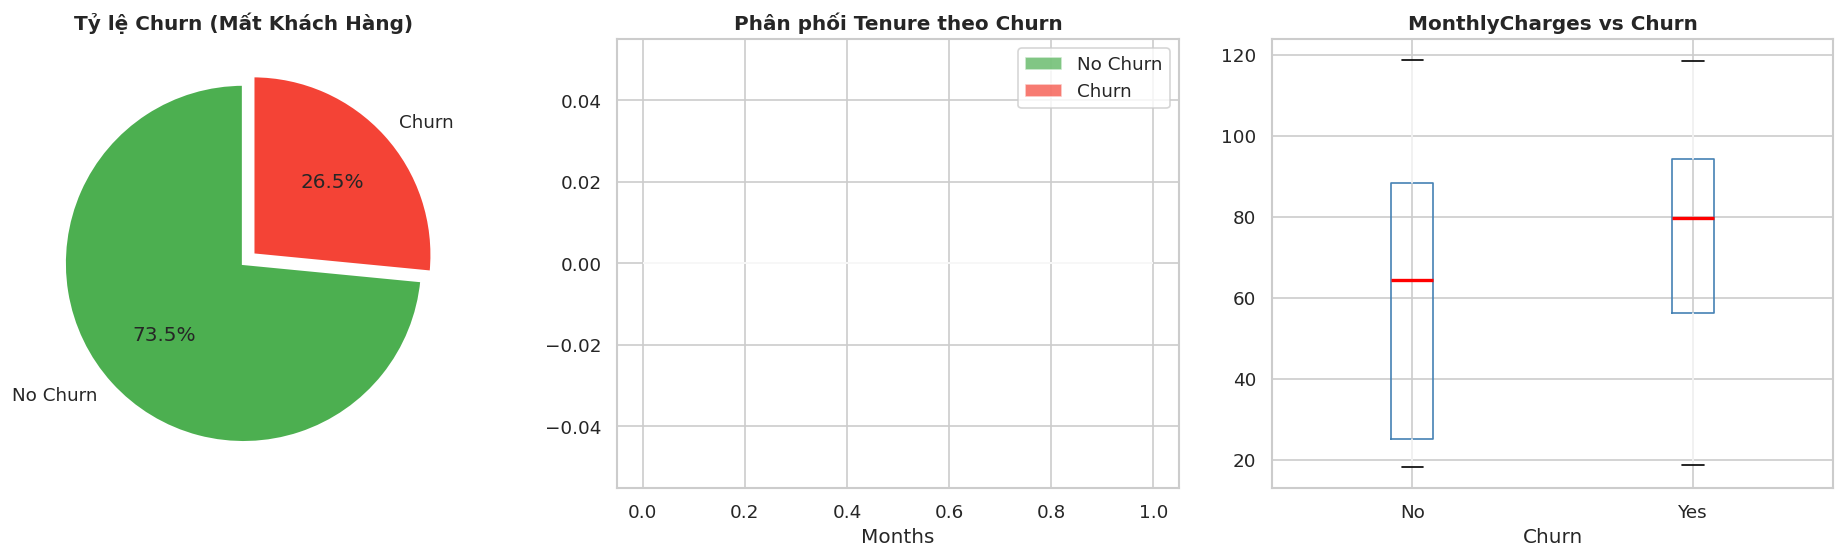
\includegraphics[width=0.9\linewidth]{Chương_1/docs/ch1/33.png}
    \caption{Kết quả EDA tổng quan: Nhận diện sự khác biệt về Tenure và Chi phí giữa hai nhóm khách hàng.}
\end{figure}

\begin{figure}[H]
    \centering
    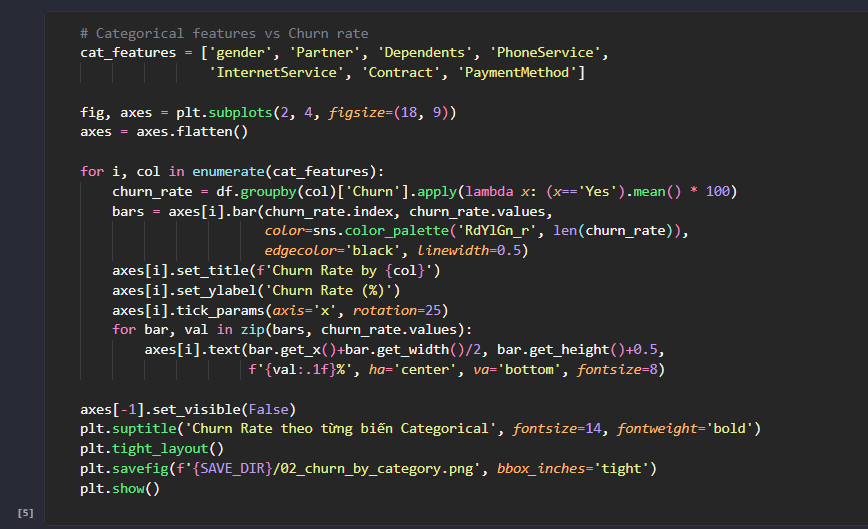
\includegraphics[width=0.9\linewidth]{Chương_1/docs/ch1/34.png}
    \caption{Mã nguồn phân tích biến hạng mục: So sánh tỷ lệ Churn theo các loại dịch vụ và hợp đồng.}
\end{figure}

\begin{figure}[H]
    \centering
    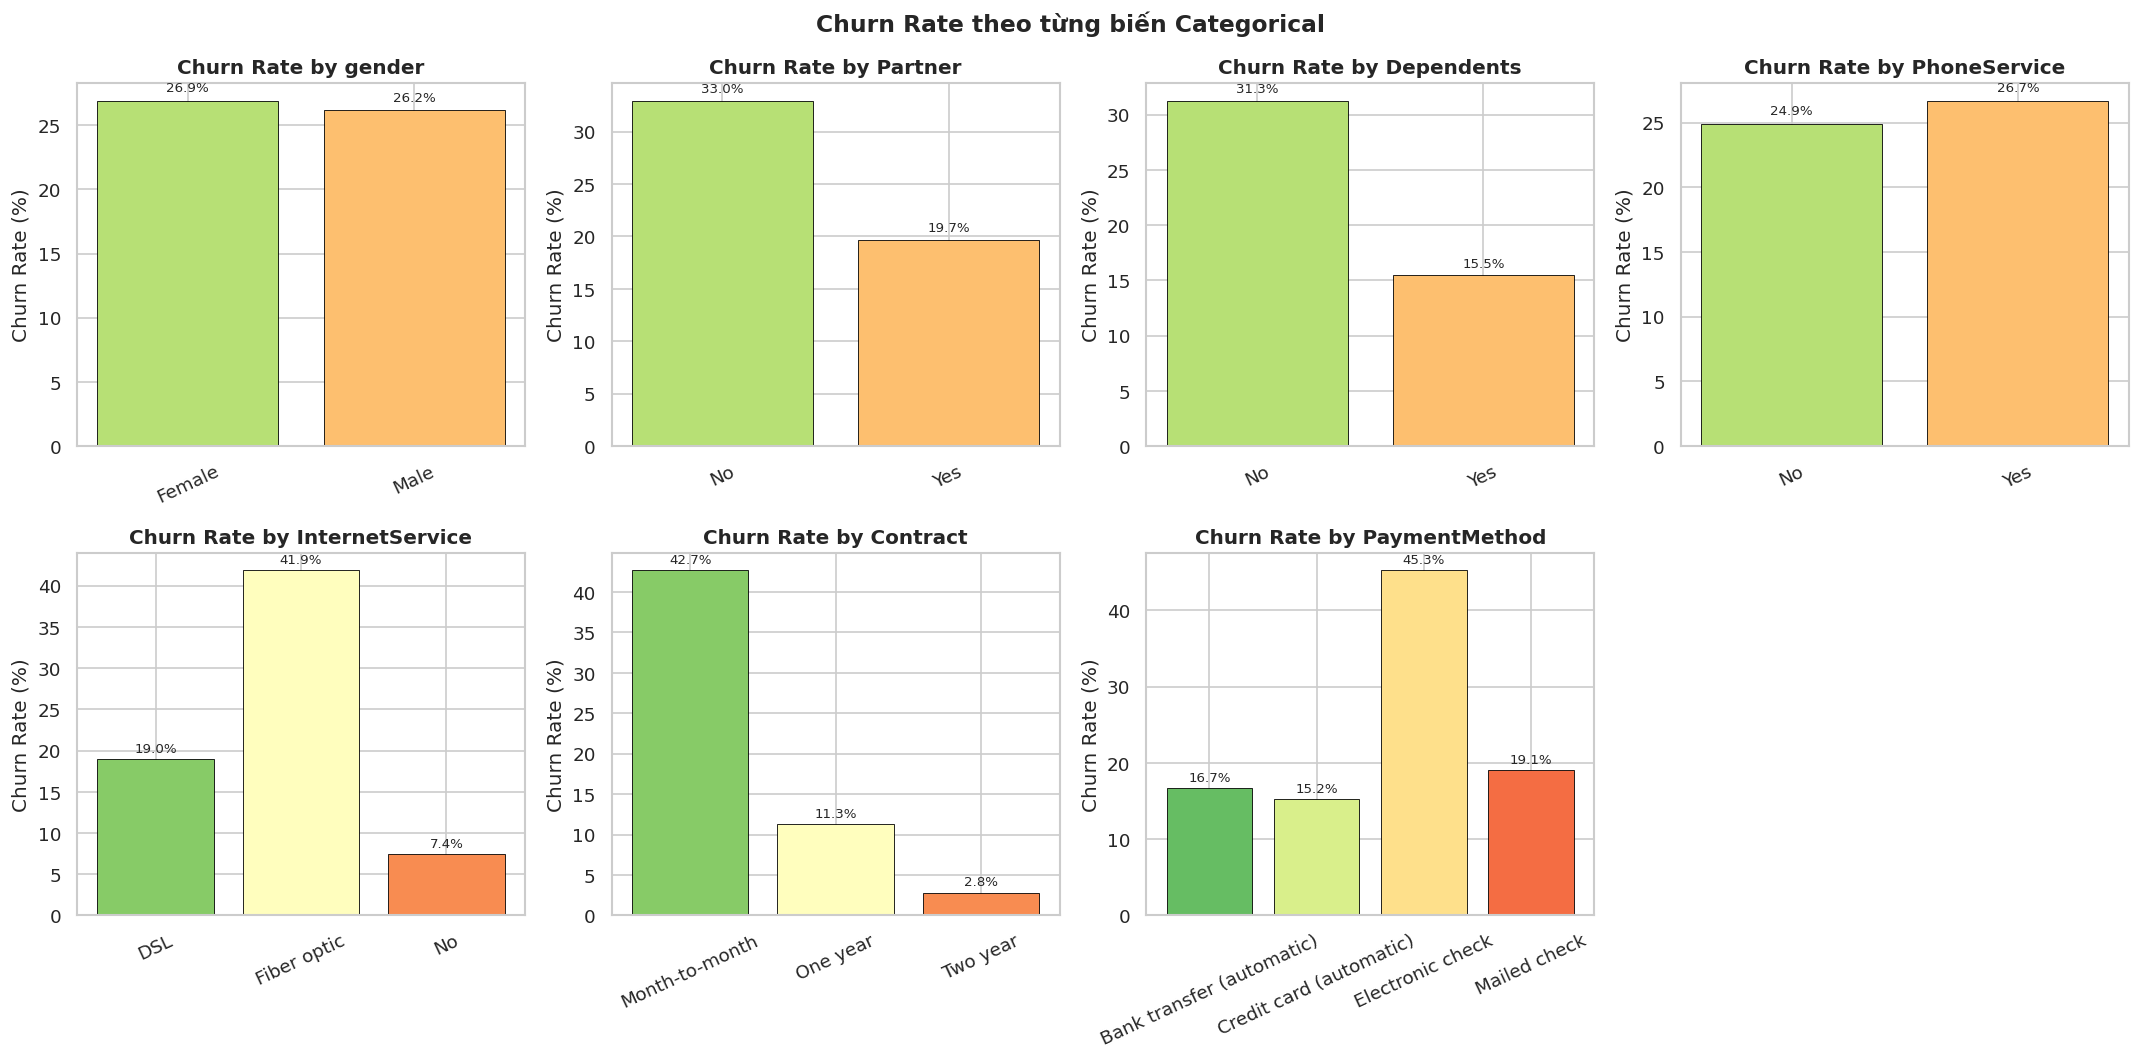
\includegraphics[width=0.9\linewidth]{Chương_1/docs/ch1/35.png}
    \caption{Kết quả phân tích hạng mục: Khách hàng dùng hợp đồng Month-to-month có tỷ lệ rời đi cao nhất.}
\end{figure}

\begin{figure}[H]
    \centering
    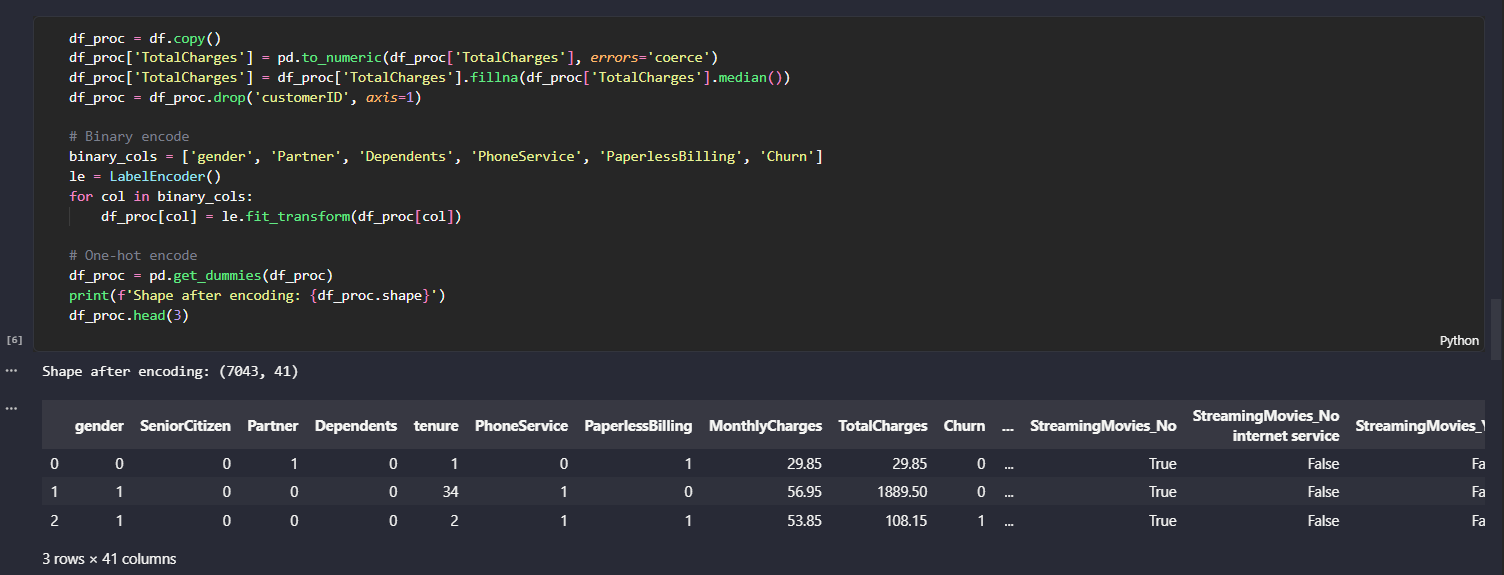
\includegraphics[width=0.9\linewidth]{Chương_1/docs/ch1/36.png}
    \caption{Mã nguồn Heatmap tương quan: Đánh giá mối liên hệ giữa các biến số sau khi mã hóa.}
\end{figure}

\begin{figure}[H]
    \centering
    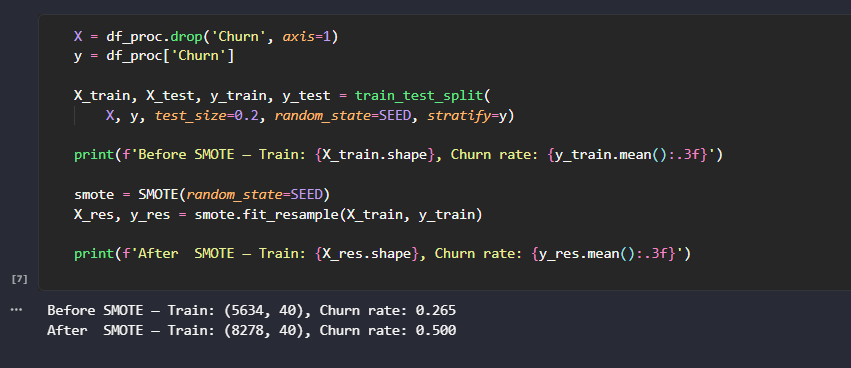
\includegraphics[width=0.9\linewidth]{Chương_1/docs/ch1/37.png}
    \caption{Kết quả Ma trận tương quan: Quan sát các biến có tương quan thuận/nghịch với Churn.}
\end{figure}

\begin{figure}[H]
    \centering
    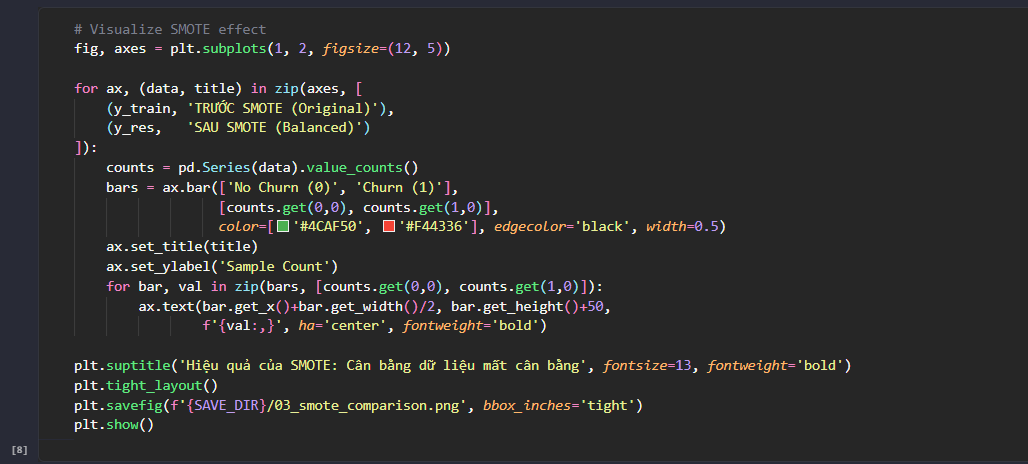
\includegraphics[width=0.9\linewidth]{Chương_1/docs/ch1/38.png}
    \caption{Tiền xử lý và SMOTE: Mã nguồn xử lý giá trị thiếu, mã hóa Label/One-hot và cân bằng dữ liệu.}
\end{figure}

\begin{figure}[H]
    \centering
    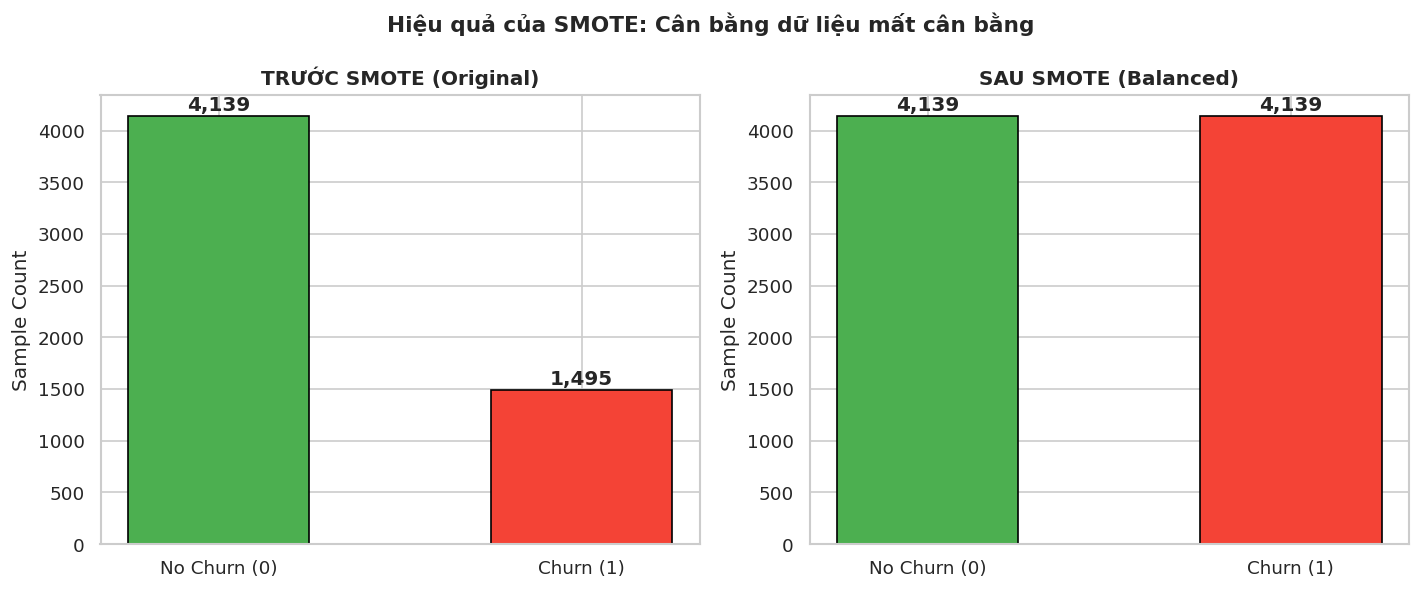
\includegraphics[width=0.9\linewidth]{Chương_1/docs/ch1/39.png}
    \caption{Kết quả SMOTE: Trực quan hóa sự thay đổi phân phối dữ liệu trước và sau khi Over-sampling.}
\end{figure}

\begin{figure}[H]
    \centering
    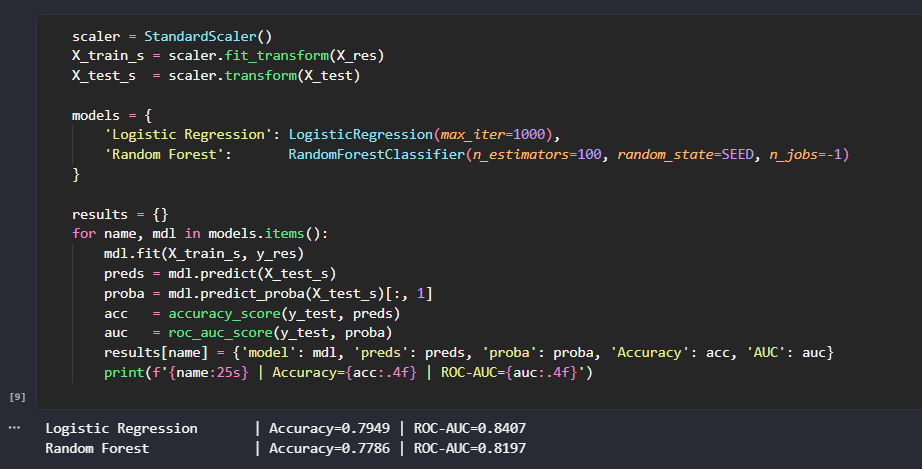
\includegraphics[width=0.9\linewidth]{Chương_1/docs/ch1/40.png}
    \caption{Huấn luyện mô hình: So sánh hiệu năng giữa Logistic Regression và Random Forest trên tập Test.}
\end{figure}

\begin{figure}[H]
    \centering
    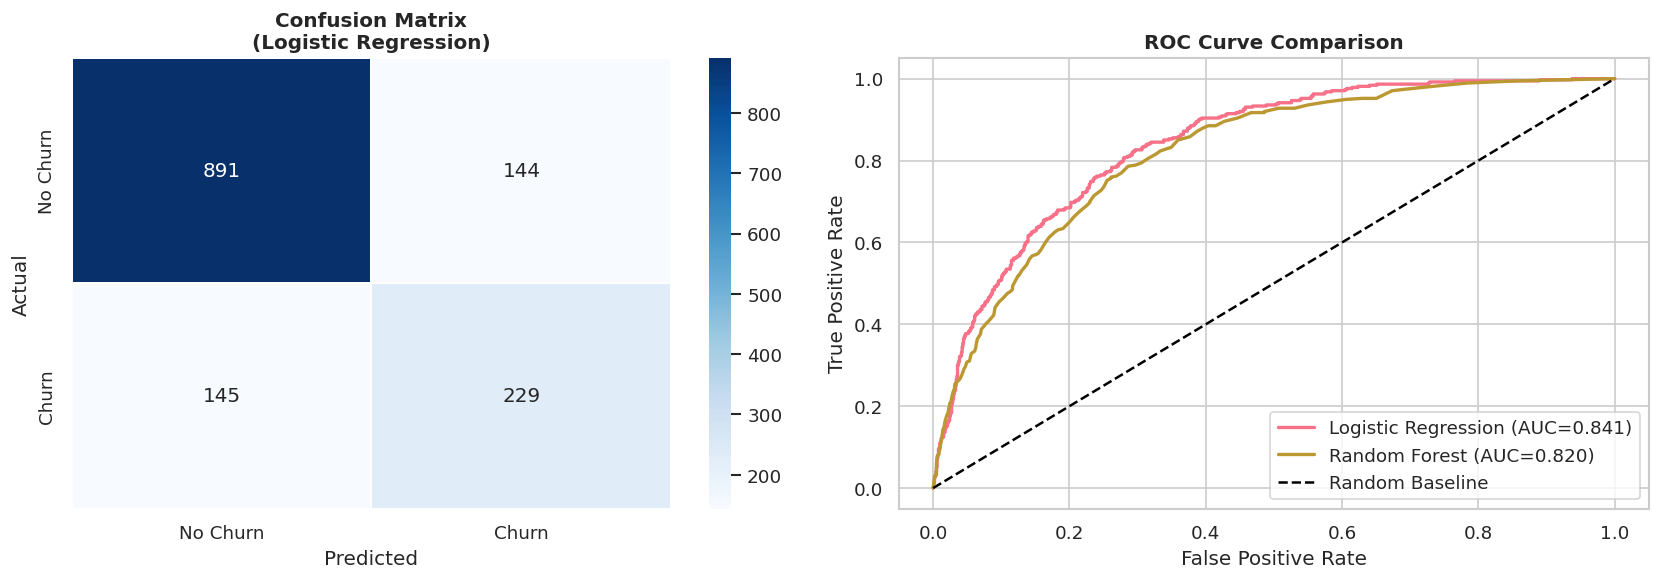
\includegraphics[width=0.9\linewidth]{Chương_1/docs/ch1/41.png}
    \caption{Mã nguồn đánh giá chi tiết: Vẽ Ma trận nhầm lẫn và đường cong ROC cho các mô hình.}
\end{figure}

\begin{figure}[H]
    \centering
    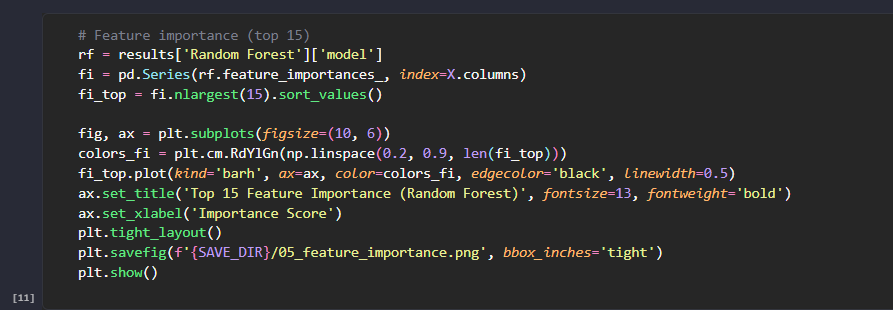
\includegraphics[width=0.9\linewidth]{Chương_1/docs/ch1/42.png}
    \caption{Kết quả đánh giá: Logistic Regression cho thấy kết quả ổn định hơn với AUC đạt 0.84.}
\end{figure}

\begin{figure}[H]
    \centering
    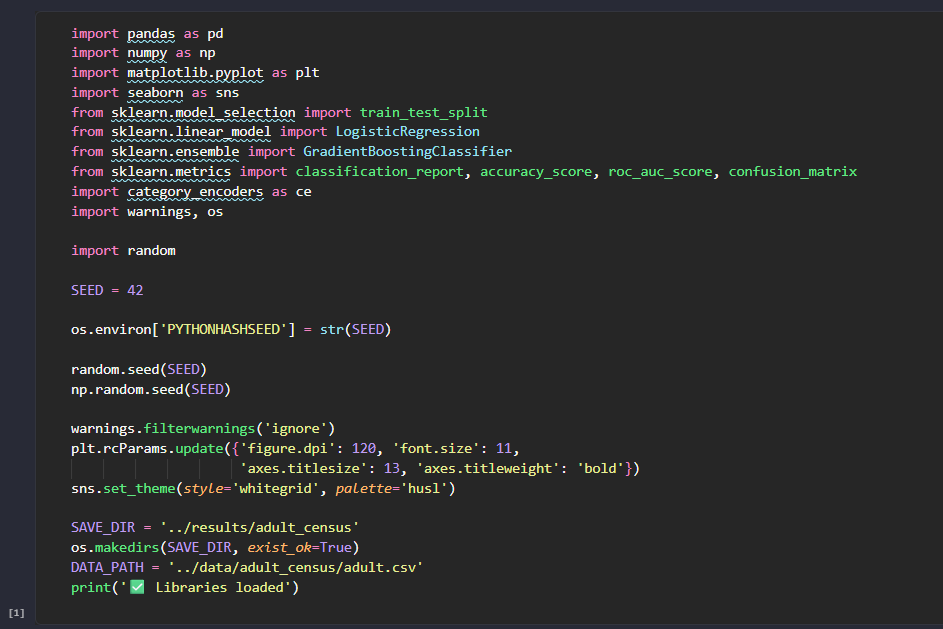
\includegraphics[width=0.9\linewidth]{Chương_1/docs/ch1/43.png}
    \caption{Tầm quan trọng của đặc trưng: Xác định các yếu tố then chốt dẫn tới quyết định rời mạng của khách hàng.}
\end{figure}
    


\subsubsection{Dataset 3: Credit Card Fraud (Anomaly - Precision-Recall Focus)}
\textbf{Thách thức:} Dữ liệu giao dịch gian lận cực kỳ hiếm (dưới 0.1%). Accuracy không còn ý nghĩa.
\textbf{Giải pháp:} Tập trung tối ưu Precision-Recall và sử dụng PCA để trực quan hóa cụm gian lận.
\paragraph{Phân tích bộ dữ liệu Credit Card Fraud} \hfill \\
Đây là bài toán cực khó với tỷ lệ dữ liệu gian lận chỉ đạt 0.172\%. Việc sử dụng Accuracy là hoàn toàn sai lầm trong ngữ cảnh này.

\paragraph{Đặc thù dữ liệu và Phân tích cấu trúc} \hfill \\
Dữ liệu đã được ẩn danh qua phép biến đổi PCA, chỉ giữ lại các cột V1-V28, cùng với thời gian (\texttt{Time}) và số tiền (\texttt{Amount}):
\begin{figure}[H]
    \centering
    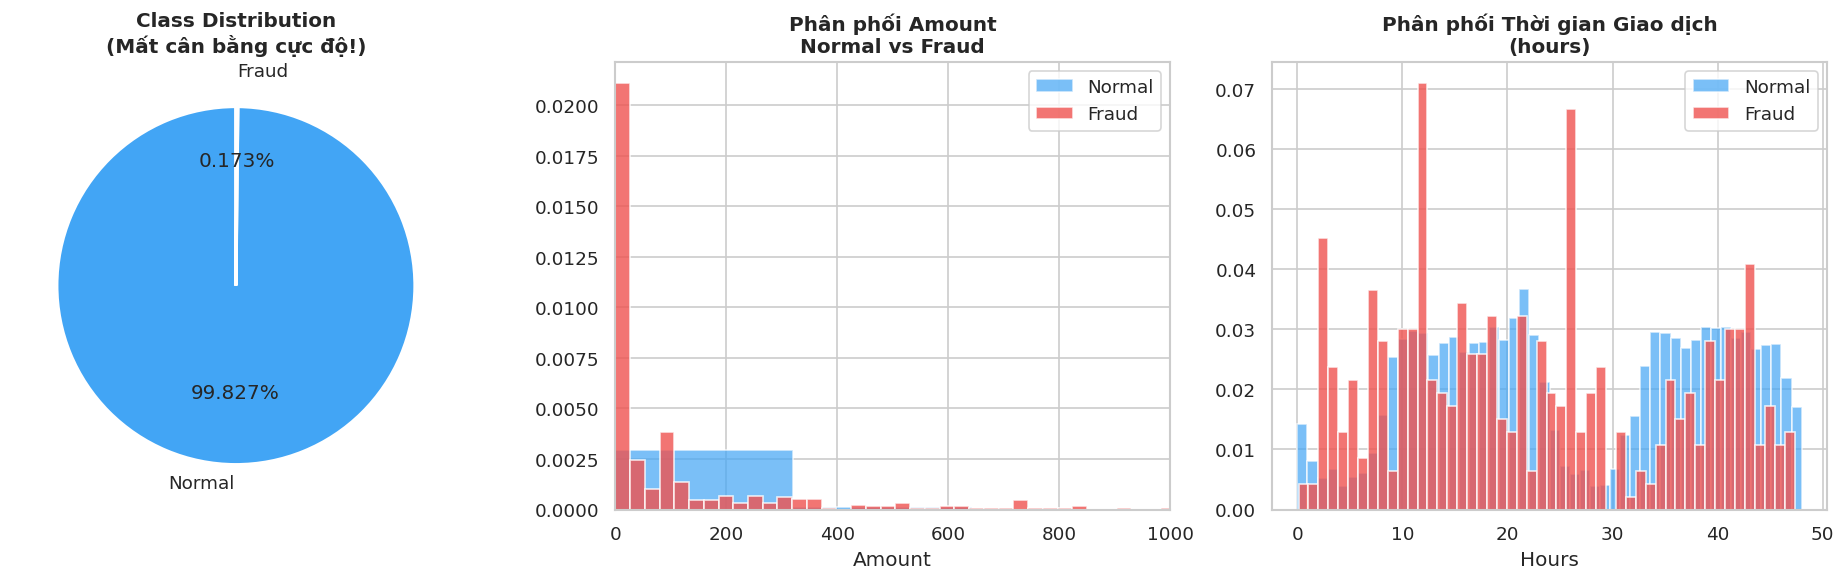
\includegraphics[width=0.8\linewidth]{Chương_1/results/credit_fraud/01_class_amount_time.png}
    \caption{Phân phối nhãn và mối liên hệ giữa Số tiền - Thời gian}
\end{figure}

Hình 1.5 cho thấy sự mất cân bằng cực độ của tập dữ liệu. Các giao dịch gian lận chiếm tỷ lệ rất nhỏ và không có sự phân hóa rõ rệt về mặt thời gian hay số tiền so với giao dịch hợp lệ, khiến việc phát hiện bằng các quy luật đơn giản là bất khả thi.

Sử dụng PCA để trực quan hóa cụm dữ liệu 2D, chúng ta thấy các vụ gian lận (màu đỏ) nằm rải rác nhưng có xu hướng tập trung ở một số vùng nhất định:
\begin{figure}[H]
    \centering
    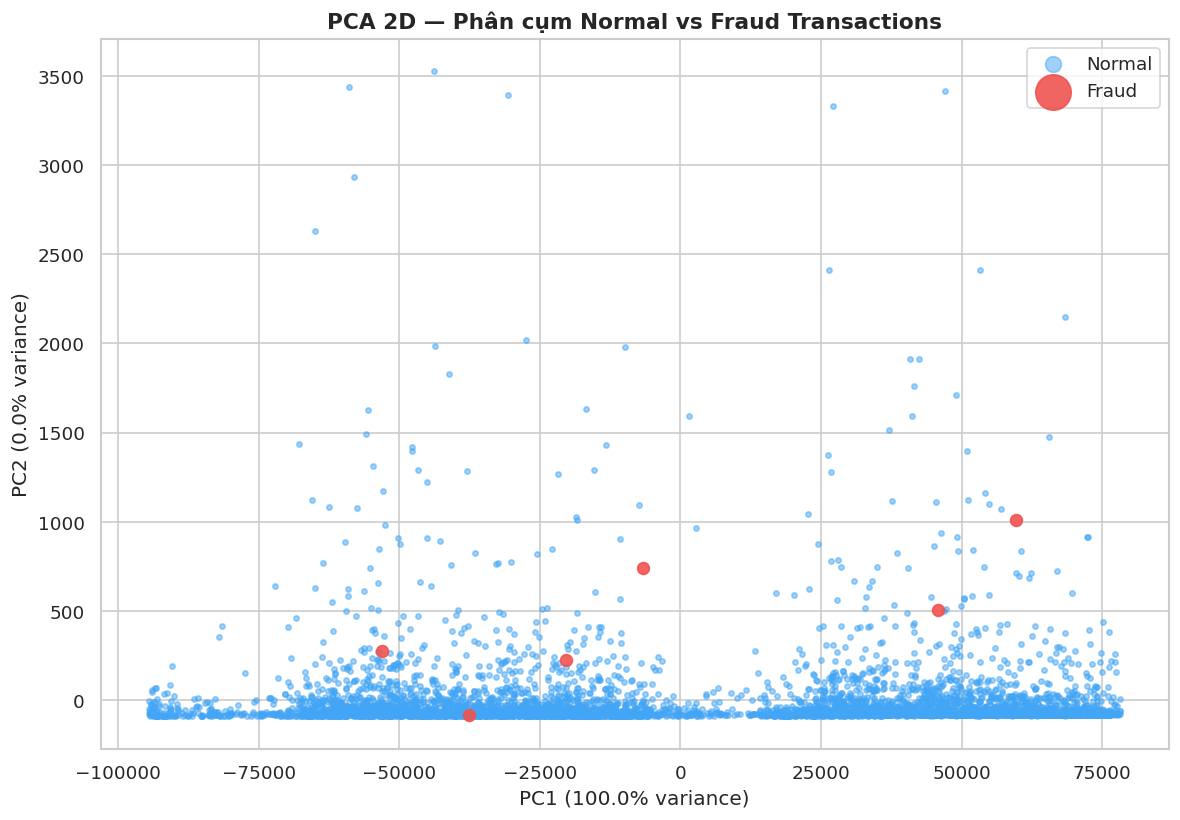
\includegraphics[width=0.8\linewidth]{Chương_1/results/credit_fraud/02_pca_2d_clusters.png}
    \caption{Trực quan hóa PCA 2D của các giao dịch}
\end{figure}

Hình 1.6 minh họa các giao dịch gian lận thông qua phép chiếu PCA xuống 2 chiều. Mặc dù có sự chồng lấn, các điểm màu đỏ (gian lận) vẫn tạo thành các cụm đặc trưng, cho phép các mô hình học máy phi tuyến tính có thể phân tách ranh giới quyết định.

Sự khác biệt về phân phối giá trị của các đặc trưng giữa giao dịch bình thường và gian lận:
\begin{figure}[H]
    \centering
    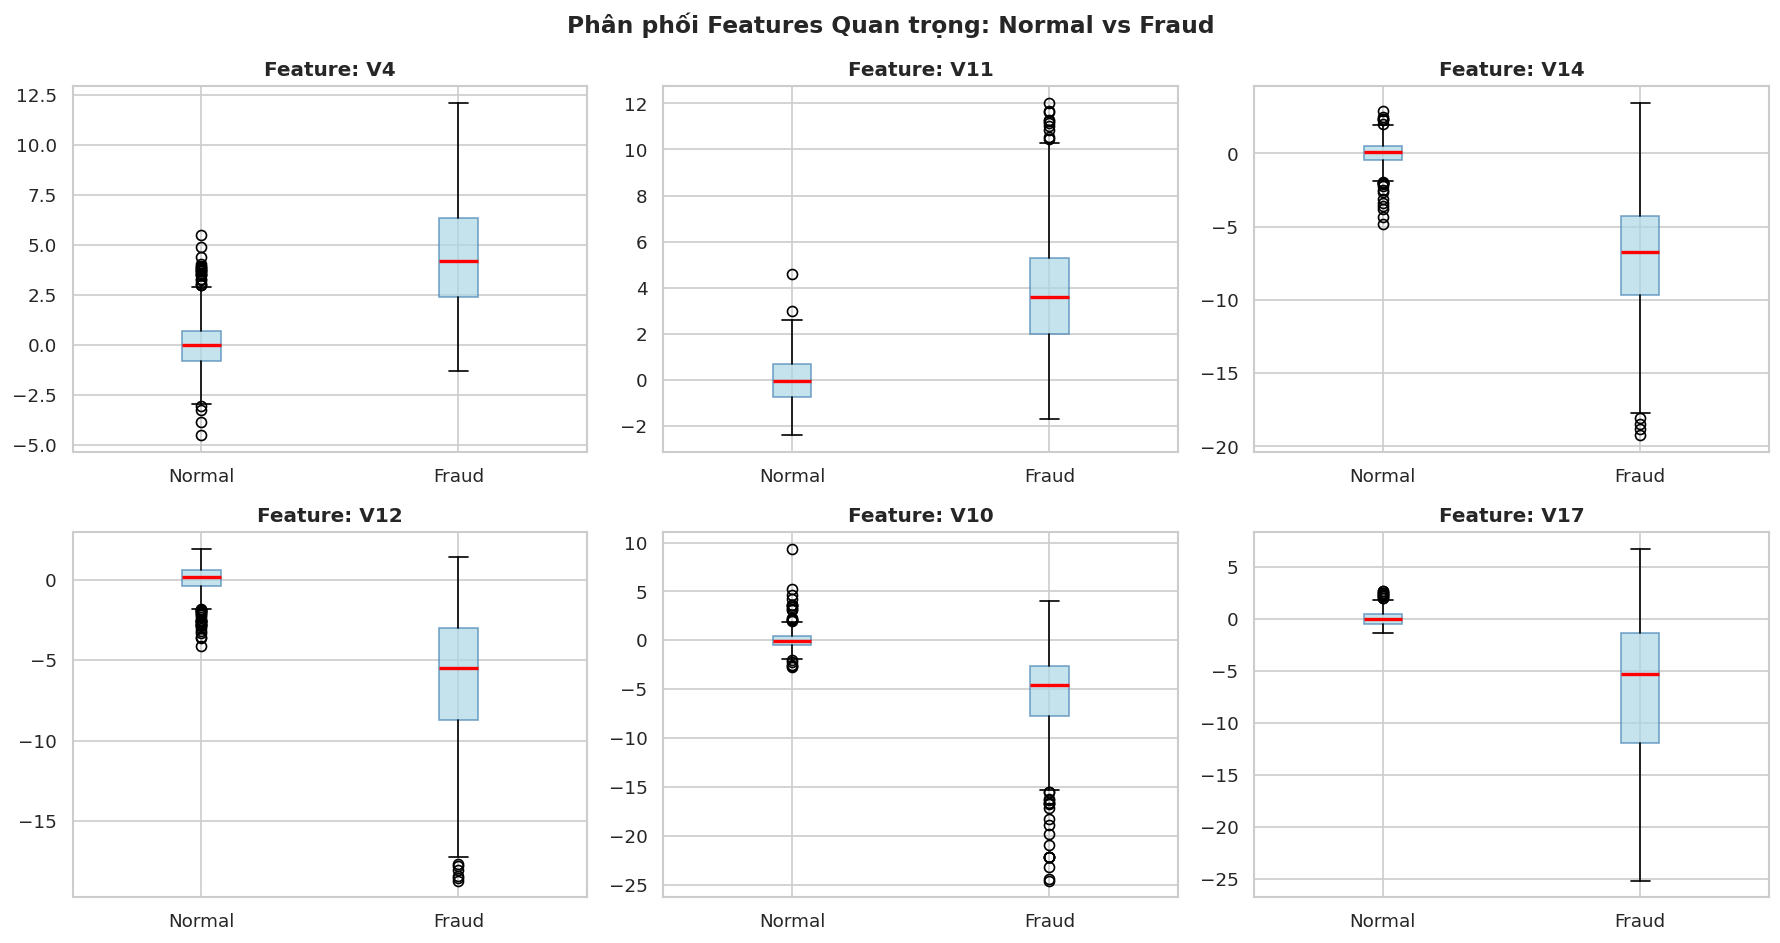
\includegraphics[width=0.8\linewidth]{Chương_1/results/credit_fraud/03_feature_boxplots.png}
    \caption{Boxplots so sánh các biến đặc trưng quan trọng}
\end{figure}

Hình 1.7 chỉ ra các biến đặc trưng có sự khác biệt lớn nhất về phân phối giữa hai lớp. Ví dụ, tại biến V14 và V17, các giao dịch gian lận thường có giá trị thấp hơn hẳn, đây là các tín hiệu quan trọng để mô hình nhận diện hành vi bất thường.

\paragraph{Kết quả thực nghiệm} \hfill \\
Chúng ta tập trung tối ưu hóa Precision-Recall (PR). Random Forest với kỹ thuật Balanced Class Weight cho kết quả rất khả thi.

\begin{table}[H]
    \centering
    \begin{tabular}{|l|c|c|c|c|}
    \hline
    \textbf{Mô hình} & \textbf{PR-AUC} & \textbf{ROC-AUC} & \textbf{Recall (Fraud)} & \textbf{Precision (Fraud)} \\ \hline
    Logistic Reg (Bal) & 0.7189 & 0.9720 & 0.92 & 0.06 \\ \hline
    \textbf{Random Forest} & \textbf{0.8653} & 0.9581 & 0.76 & \textbf{0.96} \\ \hline
    \end{tabular}
    \caption{Kết quả phát hiện gian lận (PR-AUC là chỉ số quan trọng nhất)}
\end{table}

\begin{figure}[H]
    \centering
    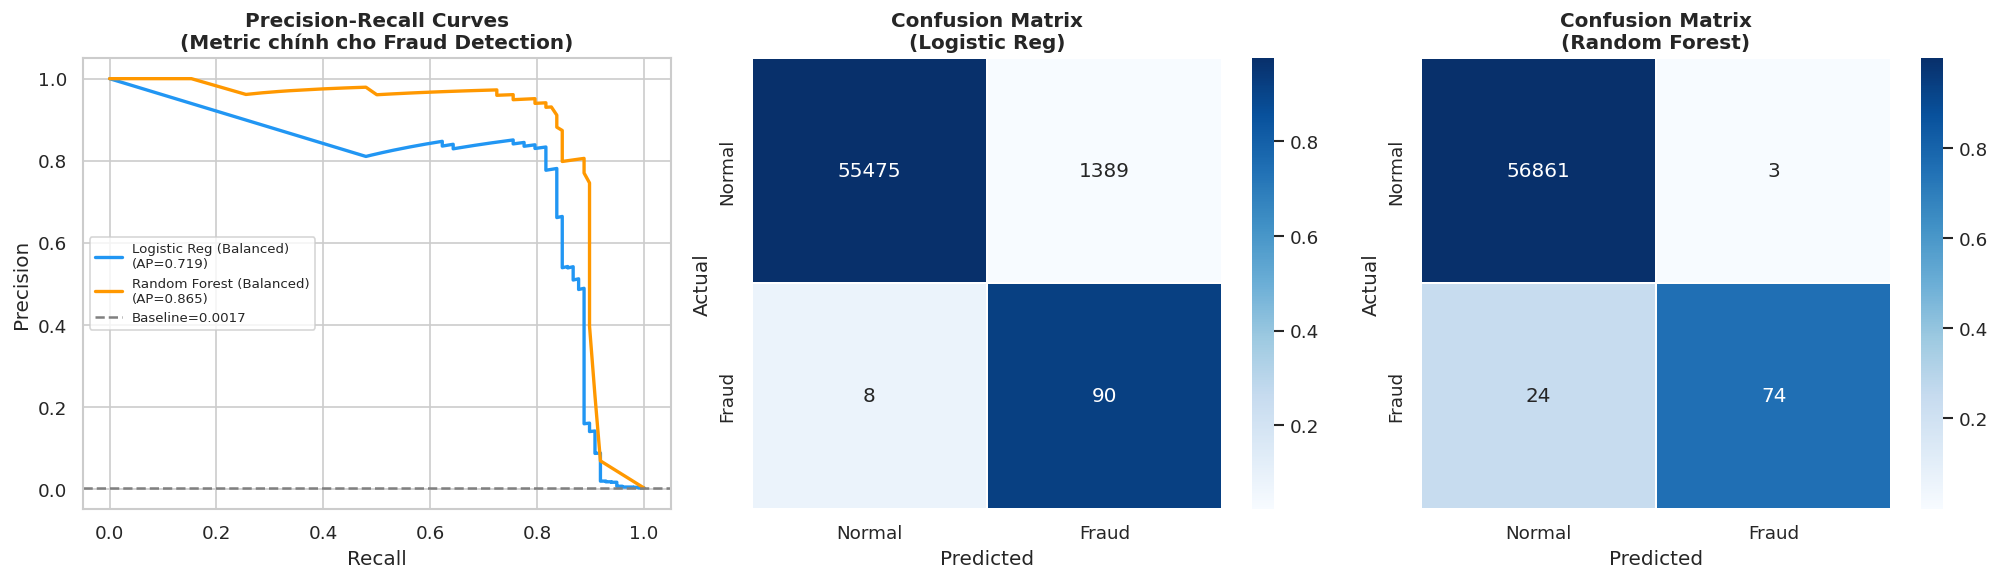
\includegraphics[width=0.8\linewidth]{Chương_1/results/credit_fraud/04_pr_curve_confusion.png}
    \caption{Đường cong Precision-Recall và Ma trận nhầm lẫn}
\end{figure}

Hình 1.8 biểu diễn đường cong Precision-Recall, một công cụ đánh giá chính xác hơn ROC trong điều kiện dữ liệu mất cân bằng. Random Forest duy trì được độ chính xác (Precision) cao ngay cả khi tăng độ bao phủ (Recall), giúp hệ thống hoạt động ổn định và tin cậy.

Random Forest đạt Precision 0.96, nghĩa là cứ 100 lần báo động gian lận thì có 96 lần là đúng, giúp giảm thiểu đáng kể chi phí kiểm tra thủ công cho ngân hàng.
    


\subsubsection{Dataset 4: Adult Census (Categorical - Target Encoding)}
\textbf{Thách thức:} Các biến như "Workclass", "Occupation" có quá nhiều nhãn, One-hot encoding sẽ làm bùng nổ số lượng cột.
\textbf{Giải pháp:} Sử dụng Target Encoding để mã hóa dựa trên xác suất của biến mục tiêu (Income >50K).
\paragraph{Phân tích bộ dữ liệu Adult Census} \hfill \\
Dữ liệu điều tra dân số năm 1994 với mục tiêu dự đoán thu nhập (>50K hay <=50K). Đặc điểm nổi bật là chứa nhiều biến định danh (Categorical) có số lượng nhãn rất lớn như "native-country" hay "occupation".

\paragraph{Kỹ thuật xử lý: Target Encoding} \hfill \\
Thay vì sử dụng One-hot Encoding (gây bùng nổ số chiều), chúng ta sử dụng Target Encoding. Kỹ thuật này thay thế mỗi nhãn bằng giá trị trung bình của biến mục tiêu tương ứng với nhãn đó. Điều này giúp mô hình nắm bắt được mối quan hệ trực tiếp giữa đặc trưng và mục tiêu mà không làm tăng độ phức tạp của dữ liệu.

\paragraph{Kết quả thực nghiệm} \hfill \\
\begin{figure}[H]
    \centering
    \includegraphics[width=0.8\linewidth]{Chương_1/results/adult_census/occupation_encoding.png}
    \caption{Xác suất thu nhập cao theo từng nhóm ngành nghề (Cơ sở của Target Encoding)}
    \label{fig:target_encoding}
\end{figure}

Việc mã hóa theo mục tiêu giúp mô hình Logistic Regression đạt được độ chính xác ổn định đồng thời giữ cho số lượng đặc trưng ở mức tối giản, giúp tăng tốc độ huấn luyện và giảm thiểu Overfitting.


\subsection{Tổng kết Chương 1}
Thông qua 4 bài toán thực tế với các thách thức khác nhau, chúng ta thấy rằng không có một quy trình tiền xử lý duy nhất cho mọi loại dữ liệu. Việc hiểu rõ bản chất của dữ liệu và lựa chọn kỹ thuật phù hợp là yếu tố tiên quyết để xây dựng mô hình AI thành công.
